% skype+baby monitor
% beamer+notebook
% esp+abs: both control brakes and motor
\subsection{Examples for Feature Interactions}

\begin{frame}{An Interaction when Customizing Clothes}
	\begin{mycolumns}[widths={66}]
		\includegraphics[width=\linewidth,page=14,trim=30 35 210 105,clip]{2021/2021-09-08-SPLC-Keynote}
	\mynextcolumn
		\begin{example}{Customization of Clothes}
			\begin{itemize}
			\item platforms such as Spreadshirt
			\item store preselects clothes with certain colors
			\item customization with pictures in different colors
			\item where is the problem?
			\end{itemize}
		\end{example}
	\end{mycolumns}
\end{frame}
\begin{frame}{An Interaction when Customizing Clothes}
	\begin{mycolumns}%[widths={40,40}]
		\myexampletight{The Problem: Unwanted Interaction of Colors}{\centering\includegraphics[width=.9\linewidth,page=15,trim=70 35 385 105,clip]{2021/2021-09-08-SPLC-Keynote}}
	\mynextcolumn
		\myexampletight{The Solution: Choose Other Colors}{\centering\includegraphics[width=.9\linewidth,page=15,trim=385 35 70 105,clip]{2021/2021-09-08-SPLC-Keynote}}
	\end{mycolumns}
\end{frame}
\begin{frame}{An Interaction when Customizing Clothes}
	\begin{mycolumns}
		\myexampletight{The Problem: Unwanted Interaction of Colors}{\centering\includegraphics[width=\linewidth,page=16,trim=50 60 360 130,clip]{2021/2021-09-08-SPLC-Keynote}}
	\mynextcolumn
		\myexampletight{The Solution: Choose Other Colors}{\centering\includegraphics[width=\linewidth,page=16,trim=360 60 50 130,clip]{2021/2021-09-08-SPLC-Keynote}}
	\end{mycolumns}
	\uncover<3->{\begin{note}{}
		\centering seems that contrast is checked for each order (cf.\ application engineering)\\and not for each published design (cf.\ domain engineering)
	\end{note}}
\end{frame}
% TODO add links to keynote?

\begin{frame}{An Interaction of Android Apps}
	\begin{mycolumns}[widths={67},animation=none]
		\only<1-2|handout:0>{\includegraphics[width=\linewidth,page=11,trim=40 30 280 100,clip]{2021/2021-09-08-SPLC-Keynote}}%
		\only<3->{\includegraphics[width=\linewidth,page=11,trim=40 30 40 100,clip]{2021/2021-09-08-SPLC-Keynote}}%
		\only<4->{\begin{note}{}%
			\centering which of those 3.5 million Android apps interact?\\where to document?\\whom to blame?%
		\end{note}}%
	\mynextcolumn
		\begin{example}{Skype vs BabyMonitor}
			\begin{itemize}
			\item Skype app installed and used for years
			\item BabyMonitor installed, carefully tried and used for months
			\item BabyMonitor can call any other number (i.e., works without internet)
			\item automatic update of the Skype app
			\item update causes a question to be asked for every call
			\item \alt<-2>{what is the problem?}{found baby crying as no one answered the dialog}
			\end{itemize}
		\end{example}
	\end{mycolumns}
\end{frame}
% TODO add links to keynote?

%\begin{frame}{Can We Trust Our Scans?}
%	\centering\includegraphics[width=\linewidth,page=28,trim=40 30 40 70,clip]{2021/2021-09-08-SPLC-Keynote}
%\end{frame}
% TODO add scanner example? is it really dependent on multiple options? or only on one particular setting

\subsection{Feature Interactions}
\begin{frame}{\myframetitle}
	\begin{mycolumns}
		\begin{definition}{Feature Interaction\mysource{\fospl\mypage{214}}}
			\mycite{A \emph{feature interaction} between two or more features is an
emergent behavior that cannot be easily deduced from the behaviors associated
with the individual features involved.}

			for short: interaction
		\end{definition}
		\begin{definition}{Unintended Interaction\mysource{\fospl\mypage{214}}}
			\mycite{An \emph{inadvertent feature interaction} occurs when a feature influences the
behavior of another feature in an unexpected way (for example, regarding the
expected control flow, program or data state, or visible behavior).}

			here: wanted vs unwanted (inadvertent)
		\end{definition}
	\mynextcolumn
		\begin{definition}{Feature-Interaction Problem\mysource{\fospl\mypage{214}}}
			\mycite{The \emph{feature-interaction problem} is to detect, manage, and resolve (inadvertent) feature interactions among features.}
		\end{definition}
		\begin{note}{Feature Interactions}
			\begin{itemize}
				\item detection discussed in next two lectures \mysource{\lectureanalyses\ and \lecturetesting}
				\item resolving interactions (see Part II)
				\item managing interactions (see Part III)
			\end{itemize}
		\end{note}
		\begin{note}{What's Next?}
			\begin{itemize}
				\item interactions due to the absence of features
				\item interactions in source code
				\item interactions with the base code
			\end{itemize}
		\end{note}
	\end{mycolumns}
\end{frame}

\begin{frame}{A Common Interaction of Toasters}
	\leftandright{
		\only<1|handout:0>{\pic[width=\linewidth]{toast1}}%
		\only<2|handout:0>{\pic[width=\linewidth]{toast2}}%
		\only<3-|handout:1>{\pic[width=\linewidth]{toast3}}%
		\uncover<5->{\myexample{}{\centering no interaction for two toasts (i.e., \emph{$T_1 \pand T_2$} shown) and for no toasts (i.e., $\pnot T_1 \pand \pnot T_2$ not shown)}}
	}{
		\only<4->{\pic[width=\linewidth]{toast4}}%
		\uncover<6->{\myexample{}{\centering unwanted interaction for one toast\\(i.e., \emph{$T_1 \pand \pnot T_2$} shown and  $\pnot T_1 \pand T_2$ not shown)}}
	}
\end{frame}

\subsection{Example Interactions with Preprocessors}
\begin{frame}{\myframetitle}
	\begin{mycolumns}[widths={75}]
		\only<1|handout:0>{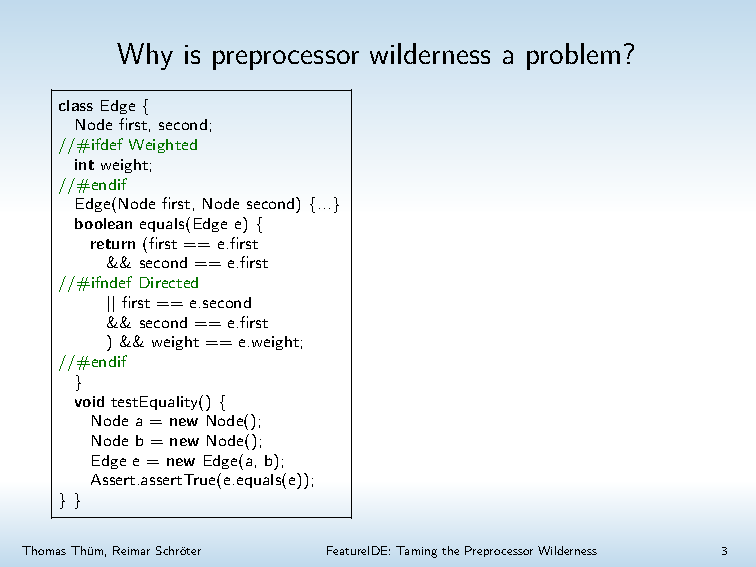
\includegraphics[width=\linewidth,page=1,trim=20 20 20 40,clip]{preprocessor-wilderness}}%
		\only<2->{\includegraphics[width=\linewidth,page=2,trim=20 20 20 40,clip]{preprocessor-wilderness}}%
	\mynextcolumn
		\begin{example}{No Interaction?}\setlength\leftmargini{3mm}
			\begin{itemize}
				\item configuration for undirected, weighted edges
				\item product can be compiled
				\item what is the problem?
			\end{itemize}
		\end{example}
	\end{mycolumns}
\end{frame}
\begin{frame}{\myframetitle}
	\begin{mycolumns}[widths={75}]
		\includegraphics[width=\linewidth,page=4,trim=20 20 20 40,clip]{preprocessor-wilderness}
	\mynextcolumn
		\begin{example}{Static Interaction}\setlength\leftmargini{3mm}
			\begin{itemize}
				\item configuration for undirected, unweighted edges
				\item product cannot be compiled due to static feature interaction
				\item field \emph{weight} used for undirected edges but defined in feature \emph{Weighted}
				\item occurs whenever features \emph{Directed} and \emph{Weighted} are both not selected
			\end{itemize}
		\end{example}
	\end{mycolumns}
\end{frame}
\begin{frame}{\myframetitle}
	\begin{mycolumns}[widths={75}]
		\includegraphics[width=\linewidth,page=3,trim=20 20 20 40,clip]{preprocessor-wilderness}
	\mynextcolumn
		\begin{example}{Other Static Interaction}\setlength\leftmargini{3mm}
			\begin{itemize}
				\item configuration for directed, weighted edges
				\item product cannot be compiled due to static feature interaction
				\item semicolon and bracket missing for every configuration with feature \emph{Directed}
				\item feature \emph{Directed} has inadvertent interaction with base code
			\end{itemize}
		\end{example}
	\end{mycolumns}
\end{frame}
\begin{frame}{\myframetitle}\setlength\leftmargini{3mm}
	\begin{mycolumns}[widths={70}]
		\includegraphics[width=\linewidth,page=5,trim=20 20 20 40,clip]{preprocessor-wilderness}
	\mynextcolumn
		\begin{example}{Dynamic Interaction?}
			\begin{itemize}
				\item again: configuration for directed, weighted edges
				\item product can be compiled but test fails
				\item not a static interaction
				\item defect in the base code
				\item no interaction at all
			\end{itemize}
		\end{example}
		\begin{note}{Detection of Interactions}
			\begin{itemize}
				\item static interactions\\\mysource{\lectureanalyses}
				\item dynamic interactions\\\mysource{\lecturetesting}
				\item next: interactions of more than two features
			\end{itemize}
		\end{note}
	\end{mycolumns}
\end{frame}

%\subsection{Unwanted and Wanted Interactions} % Desired + Undesired
% \href{https://github.com/SoftVarE-Group/Slides/blob/main/2021/2021-09-08-SPLC-Keynote.pdf}{\mycite{Every unwanted feature interaction waits to be fixed or at least documented in form of a constraint.}} T:SPLC21 

%\subsection{Pairwise Interactions}
\subsection{Higher-Order Interactions}
\begin{frame}{\myframetitle}
	\begin{mycolumns}
		\begin{definition}{Kinds of Interactions}
			\begin{itemize}
				\item wanted and unwanted interactions
				\item static and dynamic interactions
				\item one-wise interactions (interaction of features with the base code)
				\item pair-wise interactions (between two features)
				\item higher-order interactions (between more than two features)
			\end{itemize}
		\end{definition}
		\begin{example}{Variability Bug Database\mysource{\VBDb}}
			\begin{itemize}
				\item database of known feature interactions
				\item operating system Linux (43 interactions)
				\item web server Apache (23)
				\item system tool Busybox (18)
				\item 3D printer firmware Marlin (14)
			\end{itemize}
		\end{example}
	\mynextcolumn
		\myexampletight{Patterns of Feature Interactions\mysource{\VBDb}}{\pic[width=\linewidth]{variabilitybugdatabase-patterns}}
	\end{mycolumns}
\end{frame}
% TODO example from the The Variability Bug Database?

\begin{frame}{Interaction on Data and Control Flow \mytitlesource{\essentialconfigurationcomplexity}}\setlength\leftmargini{3mm}
	\begin{mycolumns}[widths={70}]
		\essentialconfigurationcomplexitylink{\includegraphics[width=\linewidth,page=2,trim=55 495 225 75,clip]{2016/2016-ASE-Meinicke}}
	\mynextcolumn
		\begin{note}{How do Features Interact?}
			\begin{itemize}
				\item given a program with runtime variability
				\item given one test case (i.e., concrete inputs)
				\item how much does the execution depend on the configuration?
				\item how many values for each variable? (green)
				\item how many different control flows? (red)
				\item blue color not relevant here (minimal overhead during simultaneous execution)
			\end{itemize}
		\end{note}
	\end{mycolumns}	
\end{frame}
\begin{frame}{Execution Traces in Configurable Systems \mytitlesource{\essentialconfigurationcomplexity}}
	\essentialconfigurationcomplexitylink{\includegraphics[width=\linewidth,page=8,trim=55 520 55 55,clip]{2016/2016-ASE-Meinicke}}

	\begin{note}{}
		\centering insights: not all features interact. some statements may lead to higher interactions than others.
	\end{note}
\end{frame}

% TODO explain duality between partial configurations and conjunctions of literals (cf. elevator product line by Varshosaz et al.)
